
\section{Sparse Grids}\label{sec:sparsegrid}

Sparse grids offer a new way to reduce the required number of grid points by order of magnitude \(O(2^{nd})\) to just only \(O(2^n n^{d-1})\) while preserving a similar error as using the full grid~\cite{Garcke2012}.
A comparison of storage requirement and error is listed in \cref{tab:comparisionfull}.
In order to achieve these bounds, the mixed second derivatives must be bounded.

The sparse grid uses a hierarchical formulation as shown in \cref{fig:basiscomp} for a one-dimensional case.
It has an incremental and adaptive behavior inherently. In order to extend to a general d-dimensional setting, it exploits
the tensor product approach.

One can use the advantage of adaptivity for problems that do not satisfy smoothness criteria or require further reduction in mesh size.
The hierarchical basis is a direct indicator of areas where further refinement is required.

\begin{figure}
    \centering
    \begin{subfigure}{0.45\textwidth}
        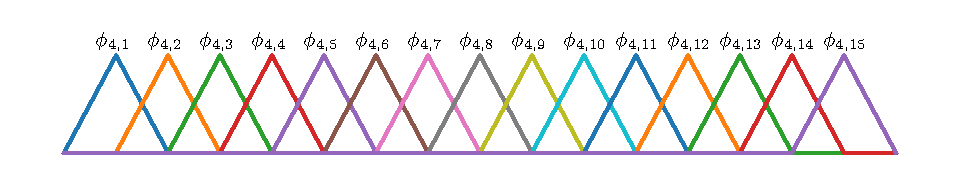
\includegraphics[width=\textwidth]{nodal_basis.pdf}
        \caption{Nodal Basis}
        \label{fig:nodalbasis}
    \end{subfigure}
    \begin{subfigure}{0.45\textwidth}
        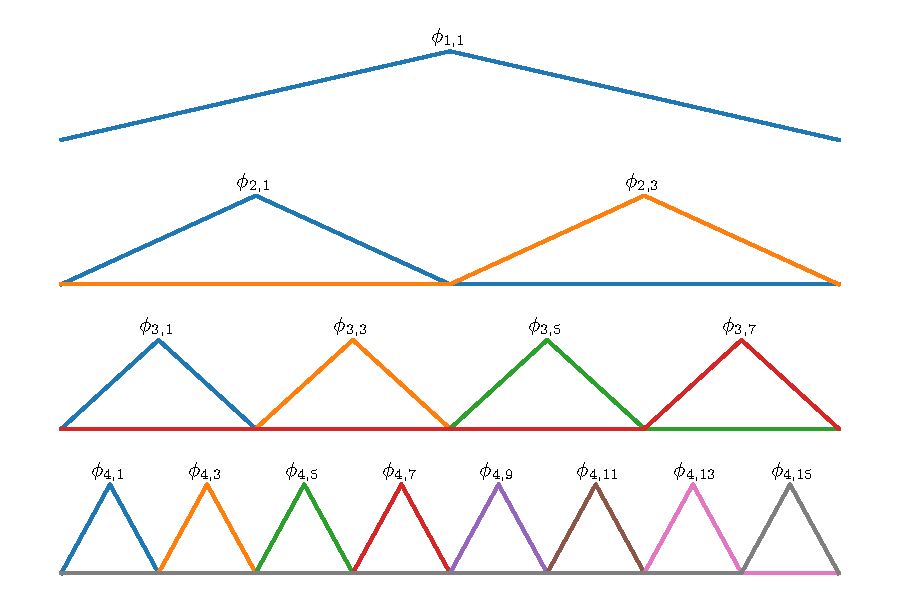
\includegraphics[width=\textwidth]{hierarchical_basis.pdf}
        \caption{Hiearchical Basis}
        \label{fig:hierarchicalbasis}
    \end{subfigure}
    \caption{Comparision of piecewise linear basis functions.}
    \label{fig:basiscomp}
\end{figure}

\begin{table}[hbpt]
    \centering
    \caption{Comparision of Sparse and Full Grid Approaches.}
    \begin{tabular}{l c c}
        \multicolumn{1}{c}{} & Storage Requirement  & \multicolumn{1}{c}{L2 Norm of Interpolation Error} \\
        \toprule
        Full Grid            & \(O(2^{nd})\)        & \(O(2^{-2n})\)                                     \\
        \midrule
        Sparse Grid          & \(O(2^{n} n^{d-1})\) & \(O(2^{-2n} n^{d-1})\)                             \\
        \bottomrule
    \end{tabular}
    \label{tab:comparisionfull}
\end{table}

In this work we will use standard hat function given by \cref{eqn:basis}.

\begin{equation}
    \phi(x ) = \left\{
    \begin{array}{ll}
        1-|x| & \text{if } x \in [-1,1] , \\
        0     & \text{otherwise}          \\
    \end{array}
    \right.
    \label{eqn:basis}
\end{equation}

On a equidistant grid \(\Omega_l \) of level \( l\) on a unit interval \(\bar{\Omega} = [0,1]\). The mesh width \(h_l\) is given by \(2^{-l} \). The grid points on a certain level is given by

\begin{equation}
    x_{l,i} = i \cdot h_l, 0 \leq i \leq 2^l
\end{equation}

Using \cref{eqn:basis} a family of basis functions \(\phi_{l,i}(x)\) with a support of \([x_{l,i}-h_l,x_{l,i}+h_l]\), by dilation and translation one could get \cref{eqn:levelbasis}. This process gives all possible basis function in level \(l\) as shown in \cref{fig:nodalbasis}.

\begin{equation}
    \phi_{l,i}(x) = \phi \left(\frac{x-i\cdot h_l}{h_l}\right)
\end{equation}

\begin{equation}
    V_l = \text{span} \left\{ \phi_{l,i} : 1 \leq i \leq 2^l-1 \right\}
    \label{eqn:levelbasis}
\end{equation}

One needs hierarchical ones in order to construct the sparse grid. The hierarchical increment spaces are given by \cref{eqn:hierarchicalincrementspace}.

\begin{equation}
    W_l = \text{span} \left\{ \phi_{l,i} : i \in I_l\right\}
    \label{eqn:hierarchicalincrementspace}
\end{equation}

where the index set is,

\begin{equation}
    I_l = \left\{ i \in \mathbb{N}: 1 \leq i \leq 2^l-1 , i \text{ odd} \right\}
\end{equation}

Using the resulting basis functions as input to the tensor product construction, one can obtain a suitable piecewise d-linear basis function at each grid point \(x_{l,i}\)

\begin{equation}
    \phi_{l,i}(x) = \prod_{j=1}^d \phi_{l_j,i_j}(x_j)
\end{equation}

More information can be found on Bungartz~\cite{Bungartz2004}.